\subsection{View implementation (Magnus)}

\textbf{Overview of files:} Each page mentioned in the View design section (\ref{sec:viewDesign}) has a corresponding JSP file, so we have: \texttt{loginPage.jsp}, \texttt{createCustomerPage.jsp}, \texttt{customerPage.jsp}, \texttt{adminPage.jsp}.
Each JSP file supports interspersed CSS, HTML and Java code. The JSP files interact with the rest of the application classes through a Servlet \texttt{DefaultServlet.java} (described in the following Control section).

\textbf{Forms:} Every user interaction is defined through an HTML \texttt{form} element. A form is a piece of code that is tied to a button, drop-down menu or similar. When a button is clicked, the form parameters are sent through a \texttt{HttpServletRequest} object to the Servlet, signalling the user's actions.

\textbf{Boxes, blocks of code:} We chose to visually collect user actions into blue/red boxes (for figures, see Appendix \ref{sec:appendixView}). This lets the user know which actions are within the same domain. The external representation (what the user sees) reflects the internal code: For each box on a page with a set of user actions, there is a block of code (specifically a HTML \texttt{div} object) in a .jsp file with corresponding form elements. e.g. the "Edit account" box contains a drop-down menu for selecting accounts (form \#1), a "set as main account" button (form \#2), and a "delete account" button (form \#3). Boxes in \texttt{customerPage} are blue, boxes in \texttt{adminPage} are red.

\begin{figure}[H]
\centering
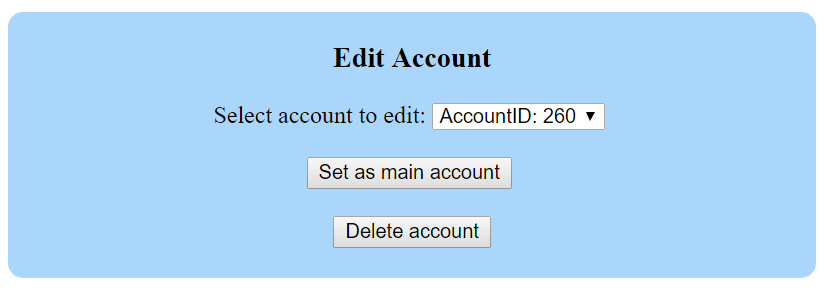
\includegraphics[width = 0.7\textwidth]{figures/forms.png}
\caption{Blue box "Edit account" in \texttt{customerPage.jsp}.}
\label{fig:forms}
\end{figure}

\textbf{HTML vs. toString:} 
When showing account information, we encountered a problem: the HTML code in jsp files ignores Java escape characters like \texttt{\textbackslash n} and \texttt{\textbackslash t}.
The solution was to  show account information in HTML tables instead. (see Fig \ref{fig:table_vs_toString}).


\textbf{Errors \& exceptions:} When a user performs an illegal action, a Java Exception is thrown internally. We implemented Exception subclasses with messages, and stored these messages in the \texttt{HttpServletRequest} object used by DefaultServlet. The error message is then displayed to the user in red text at the top of the web page. We considered using prompts, but personally found them too intrusive. How to display errors in an efficient but unobtrusive way is a subject well suited for testing.

\begin{figure}[H]
\centering
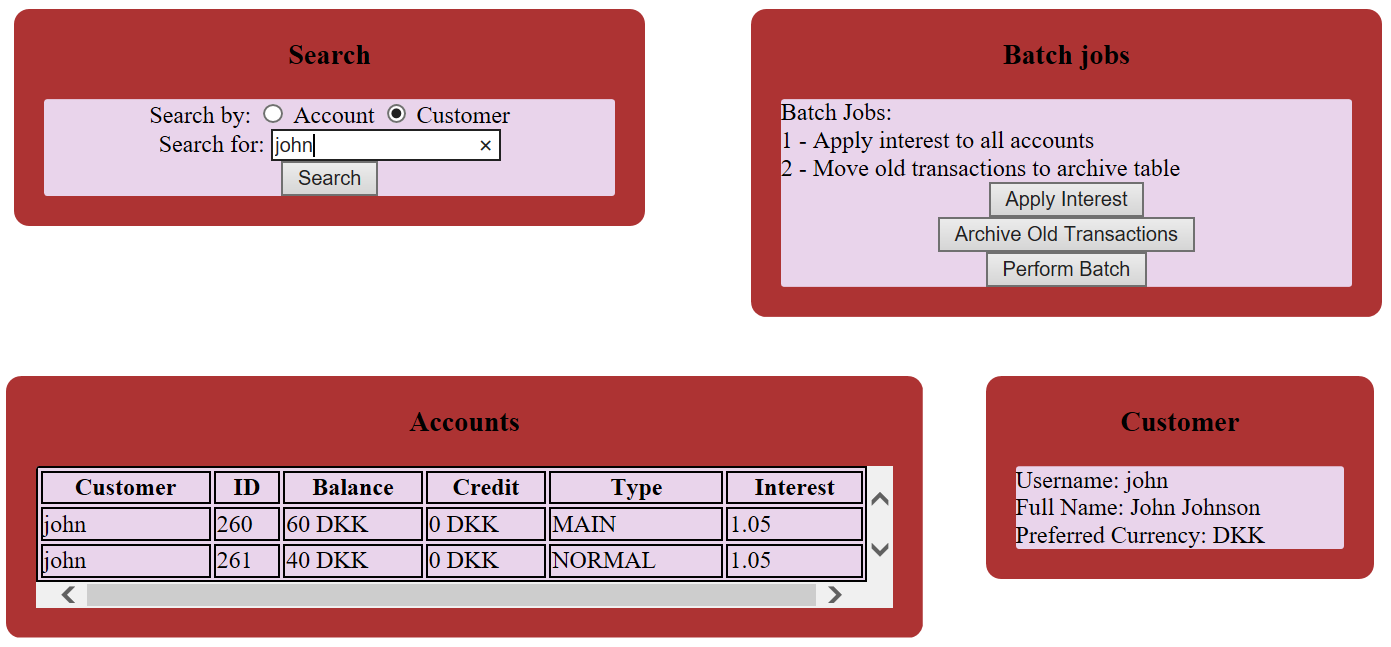
\includegraphics[width = 1.0\textwidth]{figures/adminPage_accounts.png}
\caption{An admin search for customer "john" through \texttt{adminPage.jsp}. Account information is shown in an HTML table instead of using a \texttt{toString} method. Searching by a customer by full name is not supported by the application.}
\label{fig:table_vs_toString}
\end{figure}
